% Finished August 26, 2013
% Put into VUW thesis format 29 January 2014.

\documentclass[12pt, a4paper, twoside, openright]{book}

\usepackage{vuwthesis} % sets up some local things, mostly the front page

\setlength{\intextsep}{12pt} % set space above and below in-line float
\setlength{\abovecaptionskip}{0pt} % set space between figure and caption.


%  These 3 must go before next 3, otherwise `undefined color' error may occur.
\usepackage{float}
\usepackage[usenames,dvipsnames]{xcolor}
\definecolor{litegrey}{rgb}{0.9,0.9,0.9}

\usepackage{amssymb, amsmath}
\usepackage{tikz}
\usetikzlibrary{calc}

\newcommand{\beff}{\ensuremath{b_{\mathrm{eff}}}}
\newcommand{\bmin}{\ensuremath{b_{\mathrm{min}}}}
\newcommand{\bmax}{\ensuremath{b_{\mathrm{max}}}}

%\usepackage{marvosym}

\usepackage{etoolbox}
\newtoggle{compilealone}
\toggletrue{compilealone}

\title{Chapter 7: Perturbative Effective Slip Lengths}
\author{Nat Lund}


\begin{document}
\chapter{Perturbative Effective Slip Lengths}\label{C:perturb}

We derived an expression for the effective slip length using the homogenization technique; this is presented in the previous chapter.  However, prior to doing this, we derived an expression for the effective slip length using a different technique -- the method of perturbation.  The homogenized expression for $\beff$ holds for a non-flat surface, while the perturbative expression assumes a flat surface.
% Thus, the homogenized $\beff$ subsumes the perturbative $\beff$ as a special case.
The derivation of $\beff$ by perturbation methods is presented here.

%\clearpage
\subsection{Model}

We model the fluid system as incompressible, Stokes `creeping' flow, with velocity vector $\vec{u} = (u,v,w)$: 
\begin{gather}
\nabla^2 \vec{u} = \frac{1}{\mu} \nabla p  \\
\nabla \cdot \vec{u} = 0
\end{gather}

\clearpage
The bottom solid surface is modeled as the $z=0$ plane.  
The surface is \textbf{flat,} so simple Navier slip holds:
\begin{gather}
u(0) = b(x,y) \frac{\partial u}{\partial z} \rvert_{z=0}
\end{gather}

The intrinsic slip length of the surface $b(x,y)$ is a rectangular-periodic function, with period $L$ in the $x$ direction.

The flow is Couette-like, shear-driven by a driving plate at height $P$ above the surface, with a constant driving velocity of $u_P$.
\begin{equation}
\vec{u}(x,y,P) = (u_P,0,0)
\end{equation}
Since flow is generally in the $x$ direction, driven by shear only, there is no pressure gradient, and the pressure has the same $x$-periodicity as the surface:
\begin{equation}
p(x,y,z) = p(x+L,y,z)
\end{equation}

Elements of the model are summarized in the schematic of Figure (\ref{perturbmodel}).

\begin{figure}[h]
\centering
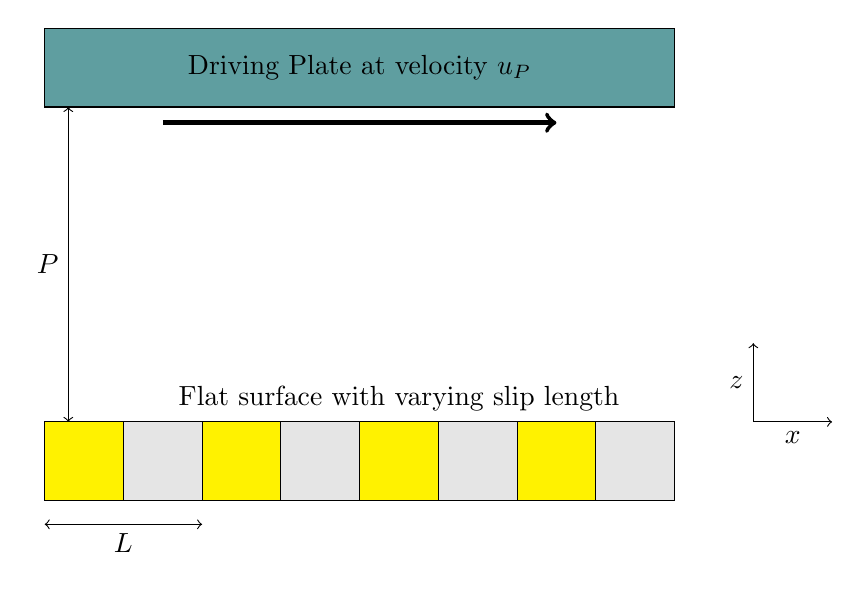
\begin{tikzpicture}

\draw[fill=CadetBlue] (0,4) rectangle node{Driving Plate at velocity $u_P$} ++(8,1);

\foreach \x in {0,2,4,6}
    {\draw[fill=yellow] (\x,0) rectangle ++(1,-1);
     \draw[fill=litegrey] (\x+1,0) rectangle ++(1,-1);}

\draw[<->] (0.3,0) -- node[left]{$P$} ++(0,4);
\draw[<->] (0,-1.3) -- node[below]{$L$} ++(2,0);

\draw[->, ultra thick] (1.5,3.8) -- ++(5,0);

\draw[<->] (9,1) -- node[left]{$z$} ++(0,-1) -- node[below]{$x$} ++(1,0);

\renewcommand{\baselinestretch}{1.00}  

\node at (4.5,0.3) {Flat surface with varying slip length}; 

\end{tikzpicture}
\caption{The model for the perturbation analyses.}\label{perturbmodel}
\end{figure}

%Note that the Navier slip condition on a flat surface is scalar, while the bulk conditions are vector equations.  This is because only the $x$ velocity slip effect is relevant to our analysis.

%Note that while the bulk conditions are vector equations, the Navier slip condition on  flat surface is scalar.  The fluid on the flat surface has no $z$ component, and we are interested in the effective slip length presented to the fluid in the far field which is shear-driven in the $x$ direction only. 

\clearpage
\section{Perturbing Plug Flow}

\subsection{Plug Flow}

Our method is to perturb an exact case of fluid flow known as plug flow, which we shall describe forthwith.  If fluid is shear-driven by a constant-velocity plate at the top boundary, and experiences \textbf{perfect slip} at the bottom boundary:
\begin{gather}
u(x,y,\mathrm{top}) = u_P \text{  (constant)} \\
\frac{\partial u}{\partial z} \rvert_{z=0} = 0
\end{gather}
then the fluid has no resistance at the bottom, so the entire bulk quickly accelerates up to velocity of the driving plate.  So fluid flows as a \textbf{plug} of fluid all at the same velocity.  This flow solution is known as plug flow, and is shown in Figure (\ref{plugflow}).

\begin{figure}[H]
\centering
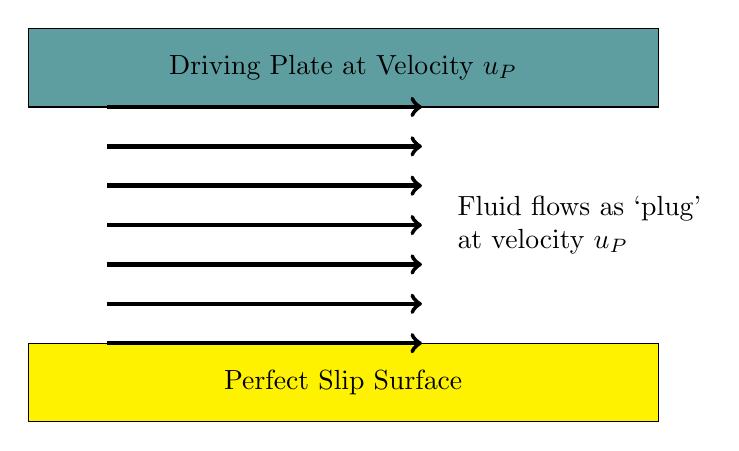
\begin{tikzpicture}
\renewcommand{\baselinestretch}{1.00}

\draw[fill=yellow] (0,0) rectangle node{Perfect Slip Surface} (8,-1);
\draw[fill=CadetBlue] (0,3) rectangle node{Driving Plate at Velocity $u_P$} ++(8,1);

\foreach \z in {0,0.5,1,1.5,2,2.5,3}
    {\draw[->, ultra thick] (1,\z) -- ++(4,0);}
    
\node at (7,1.5)[align=left] {Fluid flows as `plug'\\ at velocity $u_P$};
\end{tikzpicture}
\caption{Plug flow.} \label{plugflow}
\end{figure}

\clearpage
\subsection{Perturbed Plug Flow}

We now consider shear-driven flow that is perturbed slightly away from true plug flow.  What does it mean for a flow to be \emph{close to} plug flow?

In true plug flow, the velocity at the bottom of the fluid is the \emph{same as} the driving velocity at the top of the fluid $u_P$.  So, fluid flow is \emph{close to} plug flow if the bottom velocity is \emph{close to} the driving  velocity $u_P$.
Such plug-like flow is shown in Figure (\ref{pluglike}).

\begin{figure}[ht]
\centering
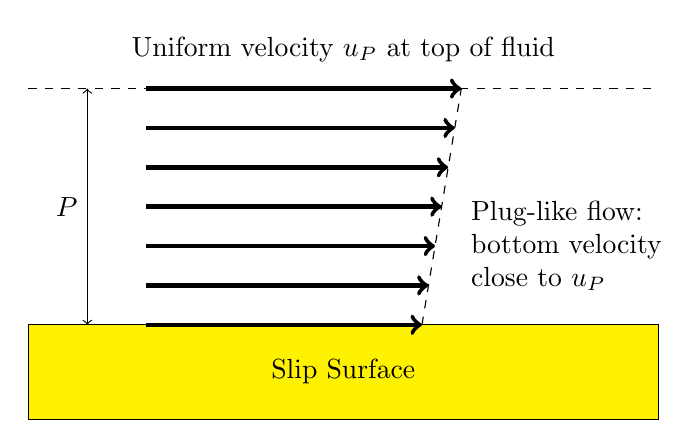
\begin{tikzpicture}
\draw[fill=yellow] (0,0) rectangle node{Slip Surface} (8,-1.2);%Patterned Slip Surface
\draw[dashed] (0,3) -- ++(8,0);
\node at (4,3.5) {Uniform velocity $u_P$ at top of fluid};
\draw[<->] (0.75,0) -- node[left]{$P$} ++(0,3);

\foreach \z in {0,0.5,1,1.5,2,2.5,3}
    {\draw[->, ultra thick] (1.5,\z) -- ++(3.5 + \z/6,0);}
    
\draw[dashed] (5,0) -- ++(0.5,3);

\renewcommand{\baselinestretch}{1.00}    
\node at (5.5,1.0)[right,align=left] 
{Plug-like flow:\\ bottom velocity\\ close to $u_P$};

\end{tikzpicture}
\caption{Plug-like flow.} \label{pluglike}
\end{figure}

If the slip surface is heterogeneous, then the slip velocity (at the bottom of the fluid) may vary across the surface.  The flow may be described as plug-like if the \emph{lowest} slip velocity is still close to $u_P$.  Since the lowest slip velocity is expected to occur over the region with the lowest intrinsic slip length, $\bmin$, flow is plug-like if $\bmin$ is sufficiently large.  By simple geometry, flow can be described as plug-like if $\bmin$ is large compared to driving height $P$, as shown in Figure (\ref{geometry}).

\clearpage

\begin{figure}[ht]
\centering
\begin{tikzpicture}
\draw (-1.5,0) -- (2.5,0);
\draw[->] (0,1) -- node[above]{$u_P$} ++(1.33,0);
\draw (0,0) -- node[left] {$P$} ++(0,1);
\draw[dashed] (0,0) -- node[left] {$\bmin$} ++(0,-6);
\draw[dashed] (0,-6) -- (1.33,1);

\end{tikzpicture}
\caption{Geometry of plug-like flow.} \label{geometry}
\end{figure}

Thus, a flow may be described as perturbed away from pure plug flow if the ratio $P/ \bmin$ is small compared to unity.  The lengths in this dimensionless ratio are fixed, measurable lengths of the physical system.  Hence, we can carry out a formal perturbation analysis with the small perturbation parameter:

\begin{equation}
\epsilon = \frac{P}{\bmin}
\end{equation}


\clearpage
\subsection{Requirement that $ L \ll P$}

The surface is patterned with a rectangular-periodic variation in slip length with period $L$ in the $x$ direction. The surface patterning causes a perturbation to the otherwise-laminar velocity profile of plug flow.  Due to the diffusion of momentum, the perturbation decays with height, so that the velocity solution converges to smooth laminar flow, as suggested in Figure (\ref{decayplug}).

\begin{figure}[h]
\centering
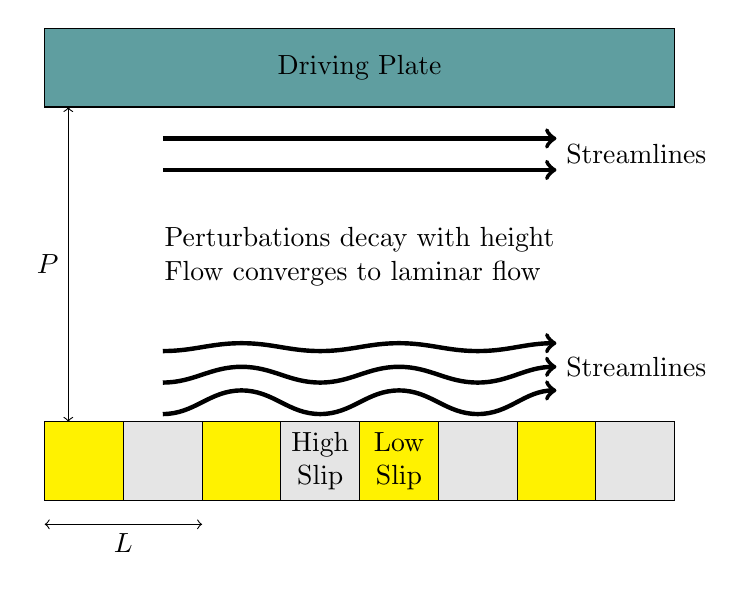
\begin{tikzpicture}

\draw[fill=CadetBlue] (0,4) rectangle node{Driving Plate} ++(8,1);

\foreach \x in {0,2,4,6}
    {\draw[fill=yellow] (\x,0) rectangle ++(1,-1);
     \draw[fill=litegrey] (\x+1,0) rectangle ++(1,-1);}

\draw[<->] (0.3,0) -- node[left]{$P$} ++(0,4);
\draw[<->] (0,-1.3) -- node[below]{$L$} ++(2,0);

\draw[->, ultra thick] (1.5,3.6) -- ++(5,0);
\draw[->, ultra thick] (1.5,3.2) -- ++(5,0);

\draw[->,ultra thick] (1.5,0.1) to [out=0,in=180] ++(1,0.3)
                              to [out=0,in=180] ++(1,-0.3)
                              to [out=0,in=180] ++(1,0.3)
                              to [out=0,in=180] ++(1,-0.3)
                              to [out=0,in=180] ++(1,0.3);

\draw[->,ultra thick] (1.5,0.5) to [out=0,in=180] ++(1,0.2)
                              to [out=0,in=180] ++(1,-0.2)
                              to [out=0,in=180] ++(1,0.2)
                              to [out=0,in=180] ++(1,-0.2)
                              to [out=0,in=180] ++(1,0.2);

\draw[->,ultra thick] (1.5,0.9) to [out=0,in=180] ++(1,0.1)
                              to [out=0,in=180] ++(1,-0.1)
                              to [out=0,in=180] ++(1,0.1)
                              to [out=0,in=180] ++(1,-0.1)
                              to [out=0,in=180] ++(1,0.1);
                              
\node at (6.5,0.7)[right]{Streamlines};
\node at (6.5,3.4)[right]{Streamlines};

\renewcommand{\baselinestretch}{1.00}    
\node at (3.5,-0.5) [align=center]{High \\ Slip};
\node at (4.5,-0.5) [align=center]{Low \\ Slip};

\node at (1.4,2.1)[right,align=left]{Perturbations decay with height \\ Flow converges to laminar flow};

\end{tikzpicture}
\caption{Plug-like flow over patterned slip with $L<P$.}\label{decayplug}
\end{figure}

Calculating the effective slip length involves finding the shear rate at the driving plate, which is assumed to be constant over the plate.  For the shear rate to be constant, the flow near the plate must be unperturbed.
%, which requires that the plate height must be greater than the decay length of the perturbation.
%  In Appendix C, we show that the decay length scales as period $L$.
In our analysis, we find that elements of the velocity perturbation are of order $ \exp(- P/L) $ at $z=P$.  These must be negliglible, which requires that:
\begin{equation}
L \ll P
\end{equation}


%Later in the analysis we show that an element of the velocity perturbation has decayed to $\exp (-P/L)$ at $z=P$.  To ensure that this quantity  is negligible at $z = P$, we require that
%\begin{equation}
%L \ll P
%\end{equation}

\clearpage



\subsection{Perturbed Navier Slip}

The Navier slip condition relates the shear rate to the slip velocity.  With $\epsilon$, we can express the slip condition as a perturbation away from shear-free plug flow.  Multiplying both sides by $\epsilon$ gives:
\begin{equation}
\frac{P}{\bmin} b(x,y) \frac{\partial u }{\partial z} = \epsilon u(0)
\end{equation}
Define the normalised slip length:
\begin{equation}
\hat{b} = \frac{b(x,y)}{\bmin},   \qquad \hat{b} \geq 1
\end{equation}
So the perturbed slip condition is:
\begin{equation}
P \hat{b} \frac{\partial u}{\partial z} = \epsilon u(0)
\end{equation}


\subsection{Perturbation Expansion}

The velocity solution to Stokes flow is assumed to be expressible as a power series in $\epsilon$:
\begin{equation}
\vec{u} = \vec{u}_0 + \epsilon \vec{u}_1 + O(\epsilon^2)
\end{equation}
where
\begin{equation}
\vec{u}_0 + \epsilon \vec{u}_1 = (u_0, v_0, w_0) + \epsilon(u_1, v_1, w_1)
\end{equation}
The pressure is similarly expressed as a power series in $\epsilon$:
\begin{equation}
p = p_0 + \epsilon p_1 + O(\epsilon^2)
\end{equation}

Both are inserted into the equations of Stokes flow with perturbed slip, giving to first order:

\begin{gather}
\nabla^2 \vec{u}_0 + \epsilon \nabla^2 \vec{u}_1 =
 \frac{1}{\mu} \nabla p_0 + \epsilon \frac{1}{\mu} \nabla p_1 \\
\nabla \cdot \vec{u}_0 + \epsilon \nabla \cdot \vec{u}_1 = 0  \\
p_0(x,y,z) + \epsilon p_1(x,y,z) = p_0(x+L,y,z) + \epsilon p_1(x+L,y,z) \\
u_0(x,y,P) + \epsilon u_1(x,y,P) = u_P \\ 
 P \hat{b} \frac{\partial u_0}{\partial z}  +
  \epsilon  P \hat{b} \frac{\partial u_1}{\partial z}
= \epsilon u_0
\end{gather}


\subsection{Zeroth Order}

By construction, setting $\epsilon$ to zero gives shear-free flow:
\begin{gather}
\nabla^2 \vec{u}_0  = \frac{1}{\mu} \nabla p_0 \\
u_0(x,y,P) = u_P \\ 
\frac{\partial u_0}{\partial z} \rvert_{z=0} = 0
\end{gather}
whose solution is plug flow.  That is, $u_0(x,y,z) = u_P$, constant everywhere.

\subsection{First Order}

Cancelling the zeroth order terms and dividing by $\epsilon$ gives the first order problem:
\begin{gather}
\nabla^2 \vec{u}_1 = \frac{1}{\mu} \nabla p_1 \\
\nabla \cdot \vec{u}_1 = 0  \\
p_1(x,y,z) = p_1(x+L,y,z) \\
u_1(x,y,P) = 0 \\ 
P \hat{b} \frac{\partial u_1}{\partial z} \rvert_{z=0} = u_0 =  u_P
\end{gather}

Note that the zeroth order solution appears in the slip condition.

\subsubsection{Eliminate Pressure with Vorticity}

The standard way to eliminate the pressure is to use the vorticity $\nabla \times \vec{u}$.
Taking the curl of both sides of the Stokes equation gives:
\begin{equation}
\nabla \times \nabla^2 \vec{u}_1  = \nabla \times \frac{1}{\mu} \nabla p_1 
\end{equation}
The right hand side is identically zero, leaving $ \nabla \times \nabla^2 \vec{u}_1 = 0 $.
Recall that the vector Laplacian is:
\begin{equation}
\nabla^2 \vec{u}_1 = \left( \nabla^2 u_1, \nabla^2 v_1, \nabla^2 w_1 \right)
\end{equation}
so that $  \nabla \times \nabla^2 \vec{u}_1 = 0 $ is
\begin{equation}
\left( 
\frac{\partial}{\partial y} \nabla^2 w_1 - \frac{\partial}{\partial z} \nabla^2 v_1,
\frac{\partial}{\partial z} \nabla^2 u_1 - \frac{\partial}{\partial x} \nabla^2 w_1,
\frac{\partial}{\partial x} \nabla^2 v_1 - \frac{\partial}{\partial y} \nabla^2 u_1
\right) = (0,0,0)
\end{equation}

This gives three PDEs.  It turns out that the successfull strategy is to use the last two. Expanding out the Laplacian operator, these are:
\begin{gather}
\frac{\partial^3 u_1}{\partial z \partial x^2} + \frac{\partial^3 u_1}{\partial z \partial y^2}
+ \frac{\partial^3 u_1}{\partial z^3} =
\frac{\partial^3 w_1}{\partial x^3} + \frac{\partial^3 w_1}{\partial x \partial y^2}
+ \frac{\partial^3 w_1}{\partial x \partial z^2} 
\\
\frac{\partial^3 u_1}{\partial y \partial x^2} + \frac{\partial^3 u_1}{\partial y^3}
+ \frac{\partial^3 u_1}{\partial y \partial z^2} =
\frac{\partial^3 v_1}{\partial x^3} + \frac{\partial^3 v_1}{\partial x \partial y^2}
+ \frac{\partial^3 v_1}{\partial x \partial z^2} 
\end{gather}
It also happens that the successful strategy is to convert the last equation into an expression in $u_1$ and $w_1$.  We can do this because the incompressibility couples $u$, $v$ and $w$.  Specifically, the continuity equation $\nabla \cdot \vec{u}_1 = 0$ can be rearranged to:
\begin{equation}
\frac{\partial v_1}{\partial y} = - \frac{\partial u_1}{\partial x} - \frac{\partial w_1}{\partial z}
\end{equation}
To use this substitution, we first differentiate the last equation with respect to $y$:
\begin{equation}
\frac{\partial^4 u_1}{\partial y^2 \partial x^2} + \frac{\partial^4 u_1}{\partial y^4}
+ \frac{\partial^4 u_1}{\partial y^2 \partial z^2} =
\frac{\partial^4 v_1}{\partial y \partial x^3} + \frac{\partial^4 v_1}{\partial x \partial y^3}
+ \frac{\partial^4 v_1}{\partial x \partial y \partial z^2} 
\end{equation}
then make the substitution, giving:
\begin{multline}
\frac{\partial^4 u_1}{\partial y^2 \partial x^2} + \frac{\partial^4 u_1}{\partial y^4}
+ \frac{\partial^4 u_1}{\partial y^2 \partial z^2} =  \\
- \frac{\partial^3 }{\partial x^3}
 \left[ \frac{\partial u_1}{\partial x} + \frac{\partial w_1}{\partial z} \right] 
- \frac{\partial^3 }{\partial x \partial y^2}
 \left[ \frac{\partial u_1}{\partial x} + \frac{\partial w_1}{\partial z} \right] 
- \frac{\partial^3 }{\partial x \partial z^2}
 \left[ \frac{\partial u_1}{\partial x} + \frac{\partial w_1}{\partial z} \right]  
\end{multline}
%\begin{multline}
%\frac{\partial^4 u}{\partial y^2 \partial x^2} + \frac{\partial^4 u}{\partial y^4}
%+ \frac{\partial^4 u}{\partial y^2 \partial z^2} =  \\
%- \frac{\partial^4 u}{\partial x^4} - \frac{\partial^4 w}{\partial x^3 \partial z} 
%- \frac{\partial^4 u}{\partial x^2 \partial y^2} 
%      - \frac{\partial^4 w}{\partial x \partial y^2 \partial z} 
%- \frac{\partial^4 u}{\partial x^2 \partial z^2} 
%      - \frac{\partial^4 w}{\partial x \partial z^3} 
%\end{multline}
Simplified:
\begin{multline}
\frac{\partial^4 u_1}{\partial x^4} 
+ 2 \frac{\partial^4 u_1}{\partial x^2 \partial y^2} 
+ \frac{\partial^4 u_1}{\partial y^4}
+ \frac{\partial^4 u_1}{\partial x^2 \partial z^2} 
+ \frac{\partial^4 u_1}{\partial y^2 \partial z^2}
=  \\
- \frac{\partial^4 w_1}{\partial x^3 \partial z} 
- \frac{\partial^4 w_1}{\partial x \partial y^2 \partial z} 
- \frac{\partial^4 w_1}{\partial x \partial z^3} 
\end{multline}

Thus we have two PDEs in two variables, $u_1$ and $w_1$.
\begin{gather}
\frac{\partial^3 u_1}{\partial z \partial x^2} + \frac{\partial^3 u_1}{\partial z \partial y^2}
+ \frac{\partial^3 u_1}{\partial z^3} =
\frac{\partial^3 w_1}{\partial x^3} + \frac{\partial^3 w_1}{\partial x \partial y^2}
+ \frac{\partial^3 w_1}{\partial x \partial z^2} 
\\
\frac{\partial^4 u_1}{\partial x^4} 
+ 2 \frac{\partial^4 u_1}{\partial x^2 \partial y^2} 
+ \frac{\partial^4 u_1}{\partial y^4}
+ \frac{\partial^4 u_1}{\partial x^2 \partial z^2} 
+ \frac{\partial^4 u_1}{\partial y^2 \partial z^2}
=
- \frac{\partial^4 w_1}{\partial x^3 \partial z} 
- \frac{\partial^4 w_1}{\partial x \partial y^2 \partial z} 
- \frac{\partial^4 w_1}{\partial x \partial z^3} 
\end{gather}


\subsubsection{Fourier Series}

Because the flow is periodic, it is natural to write $u_1$ as a Fourier series:
\begin{equation}
u_1(x,y,z) = \sum_{\vec{k}}^{\infty} U_{\vec{k}}(z) \exp(i \vec{k}\cdot \vec{r})
\end{equation}
where $\vec{r} = (x,y)$ and the wave vector $\vec{k}$ is a reciprocal lattice vector defined by integers $a$ and $b$:
\begin{gather}
\vec{k} = (m,n) = \left( \frac{ 2\pi a }{L} , \frac{ 2\pi b }{L}  \right),
 \qquad k = \frac{2 \pi q}{L} \\
\text{where} \quad k^2 = m^2 + n^2,  \quad  q^2 = a^2 + b^2
\end{gather}
The Fourier coefficient is:
\begin{equation}
U_{\vec{k}}(z) = \frac{1}{L^2} \int_0^L \int_0^L u(x,y,z) \exp(i \vec{k} \cdot \vec{r})
\;dxdy
\end{equation}
Similarly for $w_1$:
\begin{equation}
w_1(x,y,z) = \sum_{\vec{k}}^{\infty} W_{\vec{k}}(z) \exp(i \vec{k}\cdot \vec{r})
\end{equation}

The two Fourier expansions for velocity are inserted into the two PDEs.  At this point, resulting algebra was tackled with the computer package Maple.

At length, one has two expressions that are true for arbitrary $\vec{r} = (x,y)$.  As a consequence, the following two ODEs in $U$ and $W$ are true for all $\vec{k}$:
\begin{gather}
\frac{d^3 U}{dz^3} - k^2 \frac{d U}{dz} = i \left( \frac{d^2 W}{dz^2} - k^2 W \right) m 
\label{DE1} \\
k^2 \frac{d^2 U}{dz^2} - k^4 U = i \left( \frac{d^3 W}{dz^3} - k^2 \frac{dW}{dz} \right) m
\label{DE2}
\end{gather}
(The parameters $k$ and $m$ are of course not independent.)

\subsubsection{Solving the DEs}

It turns out that a successful strategy is to solve for $W(z)$ first, then substitute the solution back into Equation (\ref{DE1}), allowing us to solve for $U(z)$.

\vspace{1em}
\textbf{Solve for $W(z)$}

After multiplying Equation (\ref{DE1}) by $k^2$, and  differentiating  Equation (\ref{DE2}) with respect to $z$, the two equations may be combined to:
\begin{equation}
\frac{d^4 W}{dz^4} - 2 k^2 \frac{d^2 W}{dz^2} + k^4 W = 0
\end{equation}
The general solution of which is:
\begin{equation}
W(z) = \left( P_{\vec{k}} + Q_{\vec{k}} z \right) e^{-kz} +
\left( R_{\vec{k}} + S_{\vec{k}} z \right) e^{kz}
\end{equation}

Now, at the top of the fluid, flow is in the $x$ direction only.  Therefore $w_1(x,y,P) = 0$, which requires that
\begin{equation}
W(P) = 0
\end{equation} 

At $z=P$ the $e^{kz}$ term is $ \exp ( 2 \pi q P/L ) $ where $q \geq 1$.  Since we have assumed $P \gg L$, this term is large. Therefore we must have $R_{\vec{k}} = S_{\vec{k}} = 0$.

%The $e^{kz}$ term of $W(z)$ is obviously a problem, since $e^{kP}$ increases rapidly with increasing $P$.  Therefore we must have $R_{\vec{k}} = S_{\vec{k}} = 0$.

Furthermore, the bottom surface is impermeable, so $w_1(x,y,0) = 0$, which requires that $W(0) = 0$.  An immediate corollary is that $W(0) = P_{\vec{k}} = 0$.
We are left with:
\begin{equation}
W(z) = Q_{\vec{k}} z e^{-kz}
\end{equation} 


\textbf{Solving for $U(z)$}

We insert the solution for $W(z)$ into Equation (\ref{DE2}), yielding an ODE in $U(z)$:
\begin{equation}
\frac{d^3 U}{dz^3} - k^2 \frac{d U}{dz} = i Q_{\vec{k}} m k^2 e^{-kz} 
\end{equation}
For non-zero $k$, the general solution is:
\begin{equation}
U_{\vec{k}}(z) = \left( P_{\vec{k}} + i Q_{\vec{k}} \frac{m}{k^2} \right) e^{-kz}
+ B_{\vec{k}} e^{kz}
\end{equation}
For $k = 0$, the ODE reduces to:
\begin{equation}
\frac{d^3 U}{dz^3} = 0
\end{equation}
whose solution is:
\begin{equation}
U_0 = A_0 + B_0 z + C_0 z^2
\end{equation}


\textbf{Assemble $u_1(x,yz)$ solution}

We have found the Fourier coefficients in their most general form.  We now insert them into the Fourier series expression $ u_1(x,y,z) = \sum_{\vec{k}}^{\infty} U_{\vec{k}}(z) \exp(i \vec{k}\cdot \vec{r}) $:
\begin{gather}
u_1(x,y,z) = A_0 + B_0 z + C_0 z^2 + \sum_{k \neq 0} 
\left(  A_{\vec{k}} e^{-kz} + B_{\vec{k}} e^{kz} \right)
\exp(i \vec{k}\cdot \vec{r})\\
\text{where} \quad
A_{\vec{k}} = \left( P_{\vec{k}} + i Q_{\vec{k}} \frac{m}{k^2} \right)
\end{gather}

\textbf{Use periodicity to eliminate $C_0$}

Inserting our expression for $u_1(x,y,z)$ into the $x$ component of the Stokes equation:
\begin{equation}
\frac{\partial^2 u_1}{\partial x^2} + \frac{\partial^2 u_1}{\partial y^2} +
\frac{\partial^2 u_1}{\partial z^2} =
\frac{1}{\mu} \frac{\partial p_1}{\partial x}
\end{equation}
gives:
\begin{multline}
- m^2
\sum_{k \neq 0} 
\left(  A_{\vec{k}} e^{-kz} + B_{\vec{k}} e^{kz} \right)
\exp(i \vec{k}\cdot \vec{r})
- n^2
\sum_{k \neq 0} 
\left(  A_{\vec{k}} e^{-kz} + B_{\vec{k}} e^{kz} \right)
\exp(i \vec{k}\cdot \vec{r}) \\
+ 2 C_0
+ k^2
\sum_{k \neq 0} 
\left(  A_{\vec{k}} e^{-kz} + B_{\vec{k}} e^{kz} \right)
\exp(i \vec{k}\cdot \vec{r})
= \frac{1}{\mu} \frac{\partial p_1}{\partial x}
\end{multline}
Since $k^2 = m^2 + n^2$, this reduces to:
\begin{equation}
2 C_0 = \frac{1}{\mu} \frac{\partial p_1}{\partial x}
\end{equation}
Integrate this over one period:
\begin{gather}
\int_0^L 2 C_0 \;dx = \int_0^L \frac{1}{\mu} \frac{\partial p_1}{\partial x} \;dx \\
2 C_0 L = \frac{1}{\mu} [ p_1(L,y,z) - p_1(0,yz) ] = 0
\end{gather}
The flow is shear-driven only, so the pressure is periodic: $p_1(x,y,z) = p_1(x+L,y,z)$.  Therefore the right-hand side of the integral vanishes, and we are left with $C_0 = 0$.

\vspace{1em}
\textbf{Use top boundary condition to find $A_0$}

At the top of the fluid, the flow is uniform laminar flow with velocity $u_P$ in the $x$ direction only.  At this point, the zeroth order solution is exact, so the first order term vanishes:
\begin{equation}
u_1(x,y,P) = 0
\end{equation} 
Inserting our expression gives:
\begin{equation}
A_0 + B_0 P + \sum_{k \neq 0} 
\left(  A_{\vec{k}} e^{-kP} + B_{\vec{k}} e^{kP} \right)
\exp(i \vec{k}\cdot \vec{r})
= 0
\end{equation}

%The height $P$ of the driving plate is essentially chosen to be large enough that the $u_1(x,y,d)$ term is arbitrarily small.  This works for the $A_{\vec{k}} e^{-kd}$ term; it can be made arbitrarily small with increasing $d$.  But the $B_{\vec{k}} e^{kd}$ term gets arbitrarily \emph{large} with increasing $d$.  Therefore, we require that $B_{\vec{k}} = 0$ for all $k \neq 0$.

%The height $P$ of the driving plate may be arbitrarily large.  The $B_{\vec{k}} e^{kP}$ term gets arbitrarily large with increasing $P$.  Therefore we require that $B_{\vec{k}} = 0$ for all $k \neq 0$.  The $e^{-kP}$ can be made arbitrarily small with increasing $P$.  Then $A_{\vec{k}} e^{-kP}$ may be considered negligible; otherwise, we simply stipulate that $A_{\vec{k}} = 0$ for all $k \neq 0$.

The $e^{kP}$ term is $ \exp ( 2 \pi q P/L )$ with $q \geq 1$.  Since we have assumed $P \gg L$, this term is large. Therefore we require that $B_{\vec{k}} = 0$ for all $k \neq 0$.  
Conversely, the $e^{-kP}$ term is very small.  Then $A_{\vec{k}} e^{-kP}$ may be considered negligible; otherwise, we simply stipulate that $A_{\vec{k}} = 0$ for all $k \neq 0$.


Then the sum term is negligible or zero, and we are left with:
\begin{equation}
A_0 + B_0 P = 0
\end{equation}
from which it follows that $A_0 = - B_0 P $.  Our first-order velocity term is now:
\begin{equation}
u_1(x,y,z) =  B_0 (z - P) + \sum_{k \neq 0} 
\left(  A_{\vec{k}} e^{-kz} \right)
\exp(i \vec{k}\cdot \vec{r})
\end{equation}

\textbf{Use Slip Boundary Condition to find $B_0$}

We have found that the Fourier coefficient for $\vec{k} = (0,0)$ is $U_0 = B_0 (z - P)$.
We may equate this with the formal definition:
\begin{equation}
U_0 = B_0 (z - P) = \frac{1}{L^2} \int_0^L \int_0^L u_1(x,y,z) \;dxdy
\end{equation}
and differentiate with respect to $z$:
\begin{equation}
\frac{d}{dz} ( B_0 z - B_0 P) = \frac{1}{L^2} \int_0^L \int_0^L \frac{d}{dz} u_1(x,y,z) \;dxdy
\end{equation}
then evaluate at $z=0$:
\begin{equation}
B_0 = \frac{1}{L^2} \int_0^L \int_0^L \frac{d u_1}{dz} \rvert_{z=0} \;dxdy
\end{equation}
At this point we can substitute the slip boundary condition:
\begin{equation}
\frac{d u_1}{d z} \rvert_{z=0} = \frac{1}{P \hat{b}} u_P
\end{equation}
to get:
\begin{equation}
B_0 = \frac{1}{L^2} \int_0^L \int_0^L \frac{1}{P \hat{b}} u_P \;dxdy
\end{equation}
The double integral is the area-weighted average:
\begin{equation}
B_0 = \frac{u_P}{P} \frac{1}{L^2} \int_0^L \int_0^L \frac{1}{\hat{b}} \;dxdy
= \frac{u_P}{P} \left< \frac{1}{\hat{b}} \right>
\end{equation}

\vspace{1em}
So the \textbf{first order velocity term} is:
\begin{equation}
u_1(x,y,z) =  \frac{u_P}{P} \left< \frac{1}{\hat{b}} \right> (z - P)
 + \sum_{k \neq 0} 
\left(  A_{\vec{k}} e^{-kz} \right)
\exp(i \vec{k}\cdot \vec{r})
\end{equation}


\subsection{Bolt Together Velocity Solution}
We now have all the parts of the $x$ velocity perturbaton expansion $u(x,y,z) = u_0(x,y,z) + \epsilon u_1(x,y,z)$.  Bolting it together gives:

\begin{equation}
u(x,y,z) = u_P
 + \epsilon \frac{u_P}{P} \left< \frac{1}{\hat{b}} \right> (z - P)
 +  \epsilon \sum_{k \neq 0} 
\left(  A_{\vec{k}} e^{-kz} \right)
\exp(i \vec{k}\cdot \vec{r})
\end{equation}
Recall that:
\begin{equation}
\epsilon = \frac{P}{\bmin} \qquad \text{and} \qquad
\hat{b} = \frac{b}{\bmin}
\end{equation}
therefore:
\begin{equation}
\epsilon \frac{u_P}{P} \left< \frac{1}{\hat{b}} \right> 
= \frac{P}{\bmin} \frac{u_P}{P} \left< \frac{\bmin}{b} \right> 
= u_P \left< \frac{1}{b} \right>
\end{equation}

Thus, the final velocity solution is:
\begin{equation}
u(x,y,z) = u_P
 + u_P\left< \frac{1}{b} \right> (z - P)
 +  \epsilon \sum_{k \neq 0} 
\left(  A_{\vec{k}} e^{-kz} \right)
\exp(i \vec{k}\cdot \vec{r})
\end{equation}

\subsection{Effective Slip Length}

Since we know the height $P$ and the velocity $u_P$ of the driving plate, if we know the shear rate at the driving plate, we can calculate the effective slip length.
The flow is uniform and laminar at the driving plate, so simple shear holds, and the shear rate is simply the velocity gradient $\frac{d}{dz} u$:
\begin{equation}
\frac{d}{dz} u(x,y,z) = 
 u_P\left< \frac{1}{b} \right>
 - \epsilon \sum_{k \neq 0} 
\left( k A_{\vec{k}} e^{-kz} \right)
\exp(i \vec{k}\cdot \vec{r})
\end{equation}
At $z = P$, the term $e^{-kz} < \exp ( - 2 \pi P/L )$ and is negligible since $P \gg L$. So:
\begin{equation}
\frac{du}{dz} \rvert_{z=P} = u_P\left< \frac{1}{b} \right>
\end{equation}
Rearranging to the familiar form of Navier slip:
\begin{equation}
 u_P = \left< \frac{1}{b} \right>^{-1} \frac{du}{dz} \rvert_{z=P}
\end{equation}
%This defines the effective slip length of a virtual surface \emph{at the top of the boundary layer:
This defines an effective slip length:
\begin{equation}
\beff = \left< \frac{1}{b} \right>^{-1}
\label{eq:beff}
\end{equation}
The true slip length of the \textbf{solid surface} is less by the distance $P$ from the driving plate to the surface:
\begin{equation}
\beff = \left< \frac{1}{b} \right>^{-1} - P
\end{equation}

This result is derived by perturbing plug flow; the smallness of the perturbation is expressed by the smallness of the ratio $P/ \bmin$.  Since $ \bmin < \left< \frac{1}{b} \right>^{-1}$, the assumption $P \ll \bmin$ implies that
\begin{equation}
P \ll \left< \frac{1}{b} \right>^{-1}
\end{equation}
Therefore, the $P$ may be neglected, leaving Equation (\ref{eq:beff}).

The perturbative method has reconciled with the homogenization method: If the homogenized effective slip length formula is applied to a flat surface, it simplifies to Equation (\ref{eq:beff}).

Equation (\ref{eq:beff}) and its derivation by perturbation methods was published in 2008
 \cite{LundHendy2008}.

%Now, in the homogenization technique, we took the limit of the period of the surface patterning diminishing to zero.  This is equivalent to the limit of the thickness of the boundary layer diminishing to zero.  Therefore, the perturbed effective slip length reconciles with the homogenized slip length.
%\begin{equation}
%\lim_{d \to 0} \beff = \left< \frac{1}{b} \right>^{-1}
%\end{equation}


\clearpage
\section{Perturbed Couette Flow}

A similar analysis can be done for perturbed Couette flow.  We still assume that the height of the driving plate is much larger than the period of surface patterning :
\begin{equation}
P \gg L
\end{equation}
In this case, flow is \emph{close to} Couette flow if the maximum slip length $\bmax$ of the surface is \emph{small} compared to the height $P$ of the driving plate.  So a suitable choice of perturbation parameter is:
\begin{equation}
\epsilon = \frac{\bmax}{P}
\end{equation} 
And the normalised slip length can be defined as:
\begin{equation}
\hat{b} = \frac{b(x,y)}{\bmax}, \qquad 0 \leq \hat{b} \leq 1
\end{equation}
Then both sides of the Navier slip condition can be divided by $\epsilon$:
\begin{equation}
\frac{1}{\epsilon} u(x,y,0) = \frac{P}{\bmax} b(x,y) \frac{\partial u}{\partial z} \rvert_{z=0}
\end{equation}
So the perturbed slip condition is:
\begin{equation}
u(x,y,0) = \epsilon P \hat{b} \frac{\partial u}{\partial z} \rvert_{z=0}
\end{equation}

As before, the velocity solution is written as a perturbation expansion:
\begin{equation}
\vec{u} = \vec{u}_0 + \epsilon \vec{u}_1 = (u_0, v_0, w_0) + \epsilon(u_1, v_1, w_1)
\end{equation}
which is inserted into the Stokes, continuity, and various boundary equations.

The only difference is of course the slip condition.  To first order in $\epsilon$:
\begin{equation}
u_0 + \epsilon u_1 = \epsilon P \hat{b} \frac{\partial u_0}{\partial z} \rvert_{z=0}
\end{equation}

\subsection{Zeroth Order}

By construction, setting $\epsilon = 0$ gives classic Couette flow:
\begin{gather}
u_0(x,y,P) = u_P \\
u_0(x,y,0) = 0
\end{gather}
whose solution is a linear interpolation between the top and no-slip boundary conditions:
\begin{equation}
u_0(x,y,z) = \frac{u_P}{P} z
\end{equation}

\subsection{First Order}
Cancelling the zeroth order terms and dividing by $\epsilon$ gives the first order slip condition:
\begin{gather}
u_1 = P \hat{b} \frac{\partial u_0}{\partial z} \rvert_{z=0}
= P \hat{b} \frac{u_P}{P} \\
 u_1 = \hat{b} u_P
\end{gather}
Again, the zeroth order solution enters the slip condition.

\vspace{1em}
The analysis proceeds exactly as before, until the point where we solve for the coefficient $B_0$.
\vspace{1em}

\textbf{Use Slip Boundary Condition to find $B_0$}

We have found that the Fourier coefficient for $\vec{k} = (0,0)$ is $U_0 = B_0 (z - P)$.
We may equate this with the formal definition:
\begin{equation}
U_0 = B_0 (z - P) = \frac{1}{L^2} \int_0^L \int_0^L u_1(x,y,z) \;dxdy
\end{equation}
If we evaluate this at $z=0$, we may substitute the first order slip condition:
\begin{equation}
- B_0 P = \frac{1}{L^2} \int_0^L \int_0^L \hat{b} u_P \;dxdy
\end{equation}

The double integral is the area-weighted average:
\begin{equation}
B_0 = - \frac{u_P}{P} \frac{1}{L^2} \int_0^L \int_0^L \hat{b} \;dxdy
= - \frac{u_P }{P} \left< \hat{b} \right>
\end{equation}

\vspace{1em}
So the \textbf{first order velocity term} is:
\begin{equation}
u_1(x,y,z) =  \frac{u_P}{P} \left< \hat{b} \right> (P - z)
 + \sum_{k \neq 0} 
\left(  A_{\vec{k}} e^{-kz} \right)
\exp(i \vec{k}\cdot \vec{r})
\end{equation}

\subsection{Bolt Together Velocity Solution}
We now have all the parts of the $x$ velocity perturbaton expansion $u(x,y,z) = u_0(x,y,z) + \epsilon u_1(x,y,z)$.  Bolting it together gives:

\begin{equation}
u(x,y,z) = \frac{u_P}{P} z
 + \epsilon \frac{u_P}{P} \left< \hat{b} \right> (P - z)
 +  \epsilon \sum_{k \neq 0} 
\left(  A_{\vec{k}} e^{-kz} \right)
\exp(i \vec{k}\cdot \vec{r})
\end{equation}
Recall that:
\begin{equation}
\epsilon = \frac{\bmax}{P} \qquad \text{and} \qquad
\hat{b} = \frac{b}{\bmax}
\end{equation}
therefore:
\begin{equation}
\epsilon \frac{u_P}{P} \left< \hat{b} \right> 
= \frac{\bmax}{P} \frac{u_P }{P} \left< \frac{b}{\bmax} \right> 
= \frac{u_P}{P^2} \left< b \right>
\end{equation}
so that:
\begin{equation}
\epsilon \frac{u_P}{P} \left< \hat{b} \right> (P - z)
= \frac{u_P}{P} \left< b \right> - \frac{u_P}{P^2} \left< b \right> z
\end{equation}


Thus, the final velocity solution is:
\begin{equation}
u(x,y,z) = \frac{u_P}{P} 
\left[ z \left( 1 - \frac{\left< b \right>}{P} \right) + \left< b \right> \right]
 +  \epsilon \sum_{k \neq 0} 
\left(  A_{\vec{k}} e^{-kz} \right)
\exp(i \vec{k}\cdot \vec{r})
\end{equation}



\subsection{Effective Slip Length}

As before, we calculate the effective slip length with the velocity gradient:
\begin{equation}
\frac{\partial}{\partial z} u(x,y,z) = \frac{u_P}{P} 
\left( 1 - \frac{\left< b \right>}{P} \right)
- \epsilon \sum_{k \neq 0} 
\left( k A_{\vec{k}} e^{-kz} \right)
\exp(i \vec{k}\cdot \vec{r})
\end{equation}
%At $z$ as large as $P$, the $e^{-kz}$ term renders the sum term negligible, leaving:
At $z = P$, the term $e^{-kz} < \exp ( - 2 \pi P/L )$ and is negligible since $P \gg L$. So:
\begin{equation}
\frac{\partial}{\partial z} u(x,y,z) = \frac{u_P}{P} 
\left( 1 - \frac{\left< b \right>}{P} \right)
\end{equation}
Rearranging to the form of Navier slip:
\begin{equation}
u_P = P \left( 1 - \frac{\left< b \right>}{P} \right)^{-1}
 \frac{\partial u}{\partial z} \rvert_{z=0}
\end{equation}
Implying an effective slip length at the top boundary of:
\begin{equation}
\beff(P) = P \left( 1 - \frac{\left< b \right>}{P} \right)^{-1} 
= \frac{P}{1 - \frac{\left< b \right>}{P}}
\end{equation}

The slip length of the surface is found by subtracting $P$ from this:
\begin{gather}
\beff = \frac{P}{1 - \frac{\left< b \right>}{P}} - P \\
= \frac{P - P \left[ 1 - \frac{\left< b \right>}{P} \right]}{1 - \frac{\left< b \right>}{P}}
= \frac{ P - P + \left< b \right> }{1 - \frac{\left< b \right>}{P}} 
= \frac{\left< b \right> }{1 - \frac{\left< b \right>}{P}}
\end{gather}
We have assumed that for Couette-like flow, $\bmax \ll P$.  Clearly $\left< b \right> < \bmax $, therefore $ \left< b \right> \ll P$, and so $\left< b \right> / P$ is negligible.  We are left with:
\begin{equation}
\beff = \left< b \right>
\label{eq:bmean}
\end{equation}

(Note that for this Couette-like flow, the effective slip length `seen' at the driving plate, $\beff(P)$, is negligibly different from $P$, as expected.)

Equation (\ref{eq:bmean}) and its perturbative derivation was published in 2008 \cite{LundHendy2008}.

\clearpage
\section{Conclusion}

The effective slip length found by perturbing plug flow reconciles with the effective slip length found by homogenization.
Our perturbation analysis assumed a strict definition of plug-like flow: $P \ll \bmin$, and further assumed that near the driving plate, the perturbations had diffused into laminar flow, expressed by $L \ll P$.  In summary, the regime satisfied:
\begin{equation}
L \ll P \ll \bmin
\end{equation}

Based on this perturbation analysis, a physical regime that is \emph{close to} plug flow will have a measured effective slip length that is well approximated by the harmonic mean formula of Equation (\ref{eq:beff}): 
\begin{equation}
\beff = \left< \frac{1}{b} \right>^{-1}
\end{equation}
A system is certainly close to plug flow if $P \ll \bmin$.  However, flow may be sufficiently plug-like if the slip velocities are \emph{of the same order} as the driving velocity.  This would imply that $P \sim \bmin$.  Thus, the perturbation analysis suggests that the harmonic mean formula of Equation (\ref{eq:beff}) applies if:
\begin{equation}
L \ll P \sim \bmin
\end{equation}

This is confirmed in the numerical testing described in Chapter 8; we further discover that Equation (\ref{eq:beff}) works quite well as an approximation even when slip lengths are of the same order as the period:
\begin{equation}
L \sim b \ll P
\end{equation}

%However, the homogenization approach requires strictly that $b(x,y) > 0$.  
The perturbative approach can also be applied to the limit of vanishing slip length.  If $\bmax$ is smaller than other length scales of the flow, then the effective slip length is best approximated by the simple area-weighted average of Equation (\ref{eq:bmean}).
\begin{equation}
\beff = \left< b \right>
\end{equation}
This is confirmed by numerical simulations, as described in Chapter 8.



%\begin{center} \vspace{3em} \Coffeecup \end{center}

\iftoggle{compilealone}
    {
    \bibliography{Lund_Thesis.bib}
    \bibliographystyle{plain}
    }

\end{document}

